\documentclass[conference]{IEEEtran}
\IEEEoverridecommandlockouts
\usepackage{cite}
\usepackage{amsmath,amssymb,amsfonts}
\usepackage{graphicx}
\usepackage{textcomp}
\usepackage{booktabs}
\usepackage{array}
\usepackage{url}
\renewcommand{\ttdefault}{cmtt}

\makeatletter
\providecommand{\linebreakand}{\end{@IEEEauthorhalign}\hfill\mbox{}\par\mbox{}\hfill\begin{@IEEEauthorhalign}}
\makeatother

\begin{document}

\title{Silicon Sampling for Indian Public Opinion:\\ A Baseline-Matched Evaluation of Zero-Shot and Fine-Tuned LLMs}

\author{
\IEEEauthorblockN{Krishank Ayyella}
\IEEEauthorblockA{Department of Computer Science\\
\textit{[University Name]}\\
{}[City, Country]\\
krishankayyella@{}[domain]}
\and
\IEEEauthorblockN{Bhanuj Bhalla}
\IEEEauthorblockA{Department of Computer Science\\
\textit{[University Name]}\\
{}[City, Country]\\
bhanujbhalla@{}[domain]}
\linebreakand
\IEEEauthorblockN{Yash Bhende}
\IEEEauthorblockA{Department of Computer Science\\
\textit{[University Name]}\\
{}[City, Country]\\
yashbhende@{}[domain]}
\and
\IEEEauthorblockN{Ishaan Bansal}
\IEEEauthorblockA{Department of Computer Science\\
\textit{[University Name]}\\
{}[City, Country]\\
ishaanbansal@{}[domain]}
}

\maketitle

\begin{abstract}
Silicon sampling prompts a large language model (LLM) with a respondent's demographic profile and uses its output as that person's survey answer. We evaluate it for India on two public surveys, World Values Survey Wave~7 (WVS-7, $N{=}1{,}692$) and Pew Research Center's Religion in India survey ($N{=}29{,}999$). Every method is scored on identical respondent--item rows, supervised baselines receive the LLM's own demographic inputs, and each claim carries respondent-clustered intervals or a permutation test. Zero-shot, three LLMs (Gemini 3.1 Flash Lite, gpt-oss-120b, Qwen2.5-7B-Instruct) do not exceed the majority class on WVS-7 and trail gradient boosting (GBM) by 10 to 15 points; the majority class alone reaches 45.5\% over 144 items, leaving demographics little to add. On Pew, QLoRA fine-tuning of Qwen2.5-7B-Instruct on 184{,}853 examples reaches 36.1\% on 6{,}000 held-out respondents, 5.7 points above the majority class and 3.9 below GBM. A zero-shot control of the same model scores 17.5\%, 12.7 points below the majority class, so fine-tuning contributes 18.1 points (95\% CI 14.4--21.5). Hard predictions from the fine-tuned model and from both supervised classifiers inflate between-group differences (1.6$\times$ for the fine-tuned model, 2.0$\times$ for GBM). Subgroup gaps are reliable for religion (12.4 points) and region (8.9) and are not significantly different from GBM's, whereas at 30--40 respondents WVS gaps cannot be separated from chance; we report the detection thresholds that make this explicit.
\end{abstract}

\begin{IEEEkeywords}
silicon sampling, large language models, survey simulation, QLoRA, World Values Survey, Pew Research Center, subgroup fairness, India
\end{IEEEkeywords}

\section{Introduction}

``Silicon sampling'' conditions a language model on a sociodemographic profile and treats its output as a stand-in for that person's survey response, offering a possible low-cost complement to polling \cite{argyle2023}. Evidence that such simulations track real opinion comes largely from aggregate comparisons in the United States \cite{argyle2023,santurkar2023}, while cross-national work \cite{durmus2023} and critical re-examinations \cite{bisbee2024} indicate that fidelity varies by population and design. For India, a country of large linguistic, religious, and regional diversity, three questions decide whether the technique is usable: how accurate it is for an \emph{individual} respondent relative to a conventional model on the same demographics, whether fine-tuning on respondent-level data changes this, and whether accuracy is \emph{even} across subgroups.

We study four research questions on two public Indian surveys.
\begin{itemize}
    \item \textbf{RQ1.} Without respondent-level training data, does a zero-shot LLM predict individual answers better than simple statistics over the same demographics? (WVS-7.)
    \item \textbf{RQ2.} With such data, how does a fine-tuned LLM compare with a zero-shot control of the same model and with supervised classifiers? (Pew.)
    \item \textbf{RQ3.} How do the \emph{distributions} of predictions behave: do hard predictions keep the spread of real answers and the size of between-group differences? (Pew.)
    \item \textbf{RQ4.} Is accuracy even across subgroups, and are gaps larger than chance? (Both.)
\end{itemize}

\textbf{Contributions.}
\begin{enumerate}
    \item A \emph{baseline-matched} protocol for individual-level silicon sampling: out-of-fold scoring on identical rows, supervised baselines given exactly the prompt's features, respondent-clustered intervals, and permutation nulls with explicit detection thresholds for subgroup gaps (Section~IV).
    \item Evidence from India that LLM respondents do not exceed matched demographic baselines, from a fine-tuned model evaluated on 6{,}000 held-out Pew respondents with a zero-shot control of the same model, and from WVS-7 evaluations with three LLMs (Section~V).
    \item A distributional analysis showing that between-group inflation and concentration of hard predictions are shared by GBM and logistic regression as well as the fine-tuned LLM, so they are not specific to LLMs (Section~V-C).
    \item A reproducible pipeline and scripts to scale every experiment (Section~VIII).
\end{enumerate}

\begin{figure*}[!t]
\centering
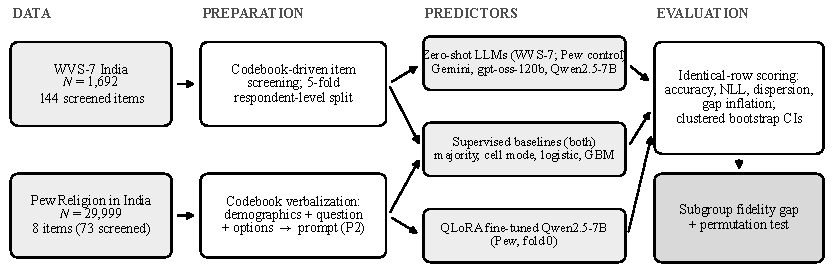
\includegraphics[width=0.98\textwidth]{figs/fig_pipeline.pdf}
\caption{Overview. Both surveys pass through codebook-driven item screening, a respondent-level 5-fold split, and shared verbalization code. WVS-7 supports zero-shot LLM evaluation; Pew supports fine-tuning and a zero-shot control. Supervised baselines are fit on both. All scoring is out-of-fold and on identical rows.}
\label{fig:pipeline}
\end{figure*}

\section{Related Work}

\textbf{Simulating survey respondents.} Argyle et al.~\cite{argyle2023} conditioned GPT-3 on sociodemographic backstories and showed that ``silicon samples'' reproduce correlations between demographics and attitudes in US data, introducing \emph{algorithmic fidelity}. Aher et al.~\cite{aher2023} replicated classic human-subject studies with LLMs, and Dillion et al.~\cite{dillion2023} discuss when models can stand in for participants. Santurkar et al.~\cite{santurkar2023} built OpinionQA from Pew surveys and found misalignment with many US demographic groups that demographic steering only partly repairs. Durmus et al.~\cite{durmus2023} found that default model responses resemble some national populations more than others. Bisbee et al.~\cite{bisbee2024} caution that synthetic responses show reduced variance and depend on prompt wording and model version. Shankar et al.~\cite{shankar2026} audit religious viewpoints across Asian populations, including India, and find minorities poorly represented.

\textbf{Fine-tuning and baselines.} Kim and Lee~\cite{kim2023} adapt language models with survey data for opinion prediction, and Suh et al.~\cite{suh2025} fine-tune them on scaled survey data to predict subpopulation response distributions. Cao et al.~\cite{cao2025} specialise LLMs to country-level response distributions from two global surveys and report partial generalisation to unseen questions and countries. WorldValuesBench~\cite{zhao2024} provides a large benchmark of WVS-derived, demographically conditioned questions. Sun et al.~\cite{sun2024} condition on group-level demographics. Krsteski et al.~\cite{krsteski2025} show that with limited human data, rectification can be more valuable than fine-tuning. Miranda and Balbi~\cite{miranda2025} compare open LLMs with random forests on ANES and find that forests match or slightly exceed the LLMs at the individual level, while the LLMs better match aggregate distributions. Chen et al.~\cite{chen2026} report, on the General Social Survey and WVS, that no LLM beats the strongest statistical baseline at the individual level, that models over-determine attitudes by demographics, and that segment gaps are inflated two- to fourfold. Ziaei~\cite{ziaei2026} reports \emph{consensus collapse}, a loss of response variance, after post-training and survey fine-tuning, most severe for non-Western countries.

\textbf{Positioning.} Our results are consistent with the individual-level conclusions of~\cite{chen2026,miranda2025} and we do not claim them as new. We add: (a)~an India-specific evaluation on two surveys, including respondent-level fine-tuning at $N\approx$ 30 thousand against matched baselines and a zero-shot control of the same model; (b)~the observation that between-group inflation and concentration of hard predictions are shared by GBM and logistic regression, so they must be interpreted against a baseline rather than as LLM-specific defects; and (c)~permutation-calibrated subgroup gaps with explicit detection thresholds, which show what sample sizes are needed to test subgroup claims.

\section{Data}

Table~\ref{tab:setup} summarises both setups.

\subsection{World Values Survey Wave 7, India}

We use the WVS-7 country-pooled file, version~6.0 \cite{wvs7}, the first release containing India ($N=1{,}692$). We parsed the official 404-page variables report into structured metadata (question wording, response scale, valid codes) and screened all 373 \texttt{Q}-prefixed columns. Items were excluded for: no codebook entry; membership in the demographic block Q260--Q290 (these condition the prompt); being a derived duplicate; insufficient scale size; nominal or non-ordinal coding; missingness above 10\%; or insufficient variation. \textbf{144 of 373} passed, and one further item (crime victimization) was removed manually as a factual-recall rather than values item. Category labels, including the eight Indian region codes, were read from the codebook annex. Zero-shot evaluation uses a fixed set of 15 of the 144 items (four are 10-point science-attitude scales).

\subsection{Pew Religion in India}

The Pew Research Center survey of religion in India \cite{pew2021} is a face-to-face survey with $N=29{,}999$ respondents. We processed the public-use file with the same pipeline: question wording and response labels were parsed from the survey's DDI metadata, and 73 items passed screening under the same rules as WVS. We use the first eight items of the frozen screened list (Fig.~\ref{fig:pewitems}a); they concern religious practice and identity, norms toward politics and abortion, sex-selective practice, and number of children, with $K=4$ to 8 answers each. Respondents are split into five folds stratified by urban/rural $\times$ income band (seed 42); this paper reports fold~0 (23{,}999 training and 6{,}000 test respondents), giving 46{,}209 evaluated (respondent, item) pairs. For subgroup analysis we use Pew's five age bands and collapse education to four bands.

\begin{table*}[!t]
\caption{Experimental setup. WVS-7 supports the zero-shot evaluations (RQ1); Pew supports fine-tuning and the zero-shot control (RQ2, RQ3). RQ4 uses both.}
\label{tab:setup}
\centering
\footnotesize
\begin{tabular}{@{}p{3.3cm}p{6.7cm}p{6.7cm}@{}}
\toprule
 & \textbf{WVS-7 India (v6.0)} & \textbf{Pew Religion in India} \\
\midrule
Respondents & 1{,}692 & 29{,}999 \\
Items screened $\rightarrow$ evaluated & 373 candidates $\rightarrow$ 144 valid $\rightarrow$ 15 evaluated & 73 valid $\rightarrow$ 8 evaluated \\
Evaluated respondents / rows & API LLMs: 30--40 respondents (421 / 556 rows); local Qwen: 120 respondents (1{,}716 rows) & fold-0 test: 6{,}000 respondents (46{,}209 rows); zero-shot control: 200 respondents (1{,}548 rows) \\
Conditioning attributes (prompt P2) & 14 (sex, age, marital status, education, employment, occupation, class, income decile, religion, urban/rural, region, town size, language, children) & 9 (sex, age band, marital status, education, religion, caste, urban/rural, region, income band) \\
LLMs & zero-shot: Gemini 3.1 Flash Lite, gpt-oss-120b, Qwen2.5-7B-Instruct & fine-tuned Qwen2.5-7B-Instruct (QLoRA, 184{,}853 examples); zero-shot Qwen2.5-7B-Instruct \\
Supervised baselines & majority, cell mode, logistic, GBM & majority, logistic, GBM \\
\bottomrule
\end{tabular}
\end{table*}

\section{Methods}

\subsection{Task, protocol, and metrics}

For respondent $i$ and item $j$, the task is to predict the respondent's actual answer category from their demographic profile and the question text. All scoring is \emph{out-of-fold}, and \emph{every comparison is made on identical (respondent, item) rows}: baselines are re-scored on exactly the rows an LLM answered. The primary metric is exact-match accuracy. We also report mean absolute error (MAE) on ordinal items, the negative log-likelihood (NLL) of the true answer where a method provides probabilities, and group-level metrics closer to how simulated respondents would be used: the \emph{subgroup-mean error} (absolute difference between predicted and true mean answer, on a scale normalised to $[0,1]$, averaged over categories with at least 100 test respondents and ordinal items), \emph{dispersion retention} (standard deviation of predictions divided by that of true answers, as in~\cite{ziaei2026}), and \emph{gap inflation} (range of predicted group means divided by range of true group means across demographic categories, median over axes and items). A reply that cannot be parsed counts as incorrect (4 of 46{,}209 Pew replies; none in WVS). Because one respondent's answers are correlated, all intervals resample respondents, not rows.

\subsection{Supervised baselines}

Per item, on training respondents, we fit (i)~the majority class (the mode of the training answers); (ii)~a demographic-cell mode on six attributes (WVS only; more attributes collapse to near-singleton cells); (iii)~multinomial logistic regression; and (iv)~histogram gradient boosting (GBM), both from scikit-learn \cite{pedregosa2011}. Logistic regression and GBM use one-hot encodings of \emph{exactly the demographics in the LLM prompt} (14 attributes for WVS, 9 for Pew), with missing codes as their own category. All baselines are mode-predicting for exact-match accuracy.

\subsection{LLM predictors}

\textbf{API models (WVS-7).} Gemini 3.1 Flash Lite (Google, free tier) and gpt-oss-120b \cite{gptoss2025} (reasoning effort ``low'', via Groq's free tier) receive a single-turn prompt (P2) with the structured demographic profile, the verbalized question, its numbered options, and an instruction to answer with one option number. Profiles and questions are rendered from codebook metadata, not hand-written, and the free-text reply is parsed against the valid codes.

\textbf{Local zero-shot Qwen2.5-7B-Instruct.} We run the same prompts through Qwen2.5-7B-Instruct \cite{qwen2025} (4-bit MLX \cite{mlx2023}, Apple M1) and read the next-token distribution over the item's option tokens, which yields both a hard prediction and probabilities (multi-token options such as ``10'' are scored by chaining token probabilities). The ``chat'' condition applies the model's chat template, the usual zero-shot usage; the ``raw'' condition feeds the bare prompt in the format the fine-tuned model was trained on. Runs use a nested random sample of respondents (fixed seed) so that conditions are comparable on identical rows. A no-demographics prompt (P0) is a single prompt per item, identical for every respondent, and isolates what the profile contributes.

\subsection{Fine-tuning (Pew)}

We fine-tune Qwen2.5-7B-Instruct with QLoRA \cite{dettmers2023}: low-rank adapters \cite{hu2022} on a 4-bit NF4 base (double quantization, bfloat16 compute). Adapters (rank 16, $\alpha{=}32$, dropout 0.05) are attached to the query, key, value, and output projections of every layer (about 10.1M trainable parameters). Each training example is the P2 prompt followed by the respondent's true answer. We train for one epoch over 184{,}853 examples (23{,}999 respondents) with effective batch size 32, peak learning rate $2\times10^{-4}$ (20 warm-up steps, linear decay), 32-bit paged AdamW, weight decay 0.01, gradient clipping 1.0, maximum sequence length 768, and seed 42 (5{,}777 steps), with the standard causal language-modelling loss over the full sequence. Training took 6.6~h (8.0~h including inference) on a single $\sim$40~GB GPU partition (transformers 5.17.0, TRL 1.13.0, PEFT 0.21.0). Test-time decoding is greedy (at most 10 new tokens) with the first valid option number parsed.

\subsection{Subgroup fidelity gap and statistical tests}

For a demographic axis $a$ with categories $\mathcal{C}_a$, the \emph{fidelity gap} of predictor $f$ is
\begin{equation}
G_a(f)=\max_{c\in\mathcal{C}_a}\operatorname{acc}_c(f)-\min_{c\in\mathcal{C}_a}\operatorname{acc}_c(f),
\end{equation}
over categories with enough data (at least 100 test respondents for Pew, 15 respondents for the WVS Qwen run, and 30 answer rows for the API-model runs). Because $G_a$ is a range, it is biased upward in small samples, so we test $H_0$: \emph{category labels are exchangeable}, by permuting labels across respondents (preserving category sizes) and recomputing $G_a$, with $p=(1+k)/(1+B)$ \cite{phipson2010}; $B=2{,}000$ (Pew) or 5{,}000 (WVS). We also report $\mathrm{Null}_{95}$, the 95th percentile of the null gap, as the smallest gap an axis can detect. Gap intervals use 1{,}000 respondent-bootstrap resamples \cite{efron1993}, accuracy and paired-difference intervals 2{,}000 to 4{,}000. Holm's correction \cite{holm1979} is applied across axes (and across models for WVS).

\section{Results}

\subsection{RQ1: zero-shot LLMs do not exceed the majority class on WVS-7}

\begin{table*}[!t]
\caption{WVS-7: LLM accuracy (\%, 95\% respondent-bootstrap CI) and each baseline's accuracy on the same rows, with the paired difference LLM $-$ baseline [95\% CI] (points). API models use 30 and 40 respondents; the local Qwen run uses a larger random sample.}
\label{tab:wvs}
\centering
\footnotesize
\setlength{\tabcolsep}{2.4pt}
\begin{tabular}{@{}lrrr@{}}
\toprule
\textbf{Row sample} & \textbf{Gemini} & \textbf{gpt-oss-120b} & \textbf{Qwen2.5-7B} \\
Respondents / rows & 30 / 421 & 40 / 556 & 120 / 1716 \\
\midrule
LLM accuracy (\%) & 25.7 [20.8, 30.5] & 23.0 [19.6, 26.7] & 22.1 [20.0, 24.4] \\
\midrule
\multicolumn{4}{@{}l}{\textit{Baseline accuracy (\%); LLM $-$ baseline [95\% CI]}} \\
Majority class & 20.9; +4.8 [$-$0.7, +10.2] & 22.3; +0.7 [$-$3.7, +5.1] & 24.9; $-$2.7 [$-$5.6, +0.1] \\
Cell mode (6 attr.) & 20.4; +5.2 [$-$0.5, +10.9] & 21.2; +1.8 [$-$2.9, +6.4] & 25.6; $-$3.4 [$-$6.5, $-$0.4] \\
Logistic (14 attr.) & 25.9; $-$0.2 [$-$5.2, +5.1] & 27.9; $-$4.9 [$-$9.4, $-$0.2] & 28.8; $-$6.7 [$-$9.9, $-$3.4] \\
GBM (14 attr.) & 35.2; $-$9.5 [$-$15.6, $-$4.4] & 34.4; $-$11.3 [$-$16.9, $-$6.2] & 37.5; $-$15.3 [$-$18.7, $-$11.9] \\
\bottomrule
\end{tabular}
\end{table*}

Across all 144 screened items, the majority class reaches 45.5\% out-of-fold accuracy and the demographic-cell mode 45.4\%, against 46.9\% for logistic regression and 50.1\% for GBM (uniform guessing: 19.4\%). Conditioning on demographics therefore adds +1.4 points (logistic) and +4.6 (GBM) over the majority class: WVS-7 India answers are concentrated and demographics are weakly informative for exact match.

On the 15 evaluated items (harder, several 10-point scales), the API models sit at the majority class and the 7B open-weight model is at or below it (Table~\ref{tab:wvs}). Gemini scores 25.7\% and gpt-oss-120b 23.0\%; relative to the majority class the paired differences are +4.8 points (95\% CI $-$0.7 to +10.2) and +0.7 ($-$3.7 to +5.1). Both are below GBM given the same attributes, by 9.5 and 11.3 points, with intervals that exclude zero. The local zero-shot Qwen2.5-7B-Instruct, evaluated on 120 random respondents (1{,}716 rows, about three times the API samples), scores 22.1\% (20.0--24.4): 2.7 points below the majority class (95\% CI $-$5.6 to +0.1), 3.4 below the cell mode, 6.7 below logistic regression, and 15.3 below GBM, with a mean NLL of 4.72 against about 1.6 for uniform guessing. The two API models agree weakly with each other (raw agreement 36.8\%, 95\% CI 32.2--41.1; Cohen's $\kappa=0.18$ \cite{cohen1960}, 0.12--0.24), and 27.6 of those 36.8 points are cases where both give the same wrong answer.

\subsection{RQ2: fine-tuning against a zero-shot control and baselines}

\begin{table}[!t]
\caption{Pew fold-0 results on 46{,}209 held-out answers from 6{,}000 respondents. $^\dagger$MAE on ordinal items. $^\S$Mean absolute error of the predicted subgroup-mean answer on a $[0,1]$ scale (hard predictions; lower is better).}
\label{tab:pewoverall}
\centering
\footnotesize
\setlength{\tabcolsep}{3pt}
\begin{tabular}{@{}lrrr@{}}
\toprule
\textbf{Method} & \textbf{Accuracy (\%) [95\% CI]} & \textbf{MAE}$^\dagger$ & \textbf{Grp. err.}$^\S$ \\
\midrule
Majority class & 30.4 [29.9, 30.8] & 1.65 & 0.34 \\
Logistic regression & 38.5 [38.0, 39.0] & 1.35 & 0.15 \\
Gradient boosting & 40.0 [39.6, 40.5] & 1.29 & 0.13 \\
Fine-tuned Qwen2.5-7B & 38.0 [37.5, 38.4] & 1.35 & 0.13 \\
\bottomrule
\end{tabular}
\end{table}

\begin{table}[!t]
\caption{Pew zero-shot control: methods scored on identical rows (200 respondents, 1{,}548 rows). FT is the fine-tuned model (hard predictions from the lab run); NLL is available for probability-producing methods.}
\label{tab:pewzs}
\centering
\scriptsize
\setlength{\tabcolsep}{3pt}
\begin{tabular}{@{}lrrr@{}}
\toprule
\textbf{Method} & \textbf{Accuracy (\%) [95\% CI]} & \textbf{NLL} & \textbf{FT $-$ method} \\
\midrule
Majority class & 30.2 [28.1, 32.4] & 1.59 & +7.5 [+5.0, +10.1] \\
Logistic regression & 38.3 [35.7, 41.0] & 1.46 & $-$0.6 [$-$2.3, +1.1] \\
Gradient boosting & 40.4 [37.3, 43.4] & 1.43 & $-$2.7 [$-$4.7, $-$0.6] \\
Zero-shot Qwen2.5-7B (chat) & 17.5 [15.7, 19.4] & 3.88 & +20.2 [+16.9, +23.5] \\
Fine-tuned Qwen2.5-7B & 37.7 [35.1, 40.3] & --- & --- \\
\bottomrule
\end{tabular}
\end{table}

Table~\ref{tab:pewoverall} gives the main full-fold result. The fine-tuned model reaches 36.1\% (95\% CI 35.6--36.6), which is $+5.7$ points over the majority class ($+5.3$ to $+6.2$), $-2.4$ relative to logistic regression, and $-3.9$ relative to GBM ($-4.4$ to $-3.5$); it closes 59\% (55--63\%) of the distance between the majority class and GBM. Baseline accuracy is stable across folds (GBM 39.6--40.4\%, majority 29.7--30.4\%). Per item (Fig.~\ref{fig:pewitems}a) the fine-tuned model exceeds the majority class on seven of eight items, each with an interval excluding zero, and trails GBM on every item by 1.7 to 10.4 points.

\textbf{Zero-shot control.} Table~\ref{tab:pewzs} compares the methods on a nested random sample of 200 test respondents (1{,}548 rows). The fine-tuned model scores 35.6\% here against 36.1\% on the full fold, so the subset is representative. The zero-shot model with the chat template scores 17.5\% (95\% CI 15.7--19.4), 12.7 points \emph{below} the majority class (30.2\%) and at the level of uniform guessing (19.4\%). Fine-tuning raises accuracy by 18.1 points (paired 95\% CI 14.4 to 21.5). The zero-shot model is also poorly calibrated: its mean NLL is 3.88, against 1.59 for the majority class, because nearly all of its probability mass sits on one moderate option. A label-free prior correction (rescaling its probabilities by the training-set marginal divided by its own mean prediction) lifts it to 26.3\% (24.0--28.6), still below the majority class and 9.3 points (6.0 to 12.6) below the fine-tuned model, so the gain from fine-tuning is not merely a corrected item-level prior. The raw prompt format used in fine-tuning gives the same picture (120-respondent subset: 18.8\%, 15.9--21.8; 12.0 points below the majority class). Removing the demographic profile altogether (P0) gives \emph{higher} zero-shot accuracy, 21.1\% (19.1--23.1), than with it: adding the profile changes accuracy by $-$3.6 points ($-$5.9 to $-$1.2). The model does react to the profile, since its answer changes on 50\% of rows (a different prediction in the other half), but not in a way that improves exact-match accuracy.


\begin{figure*}[!t]
\centering
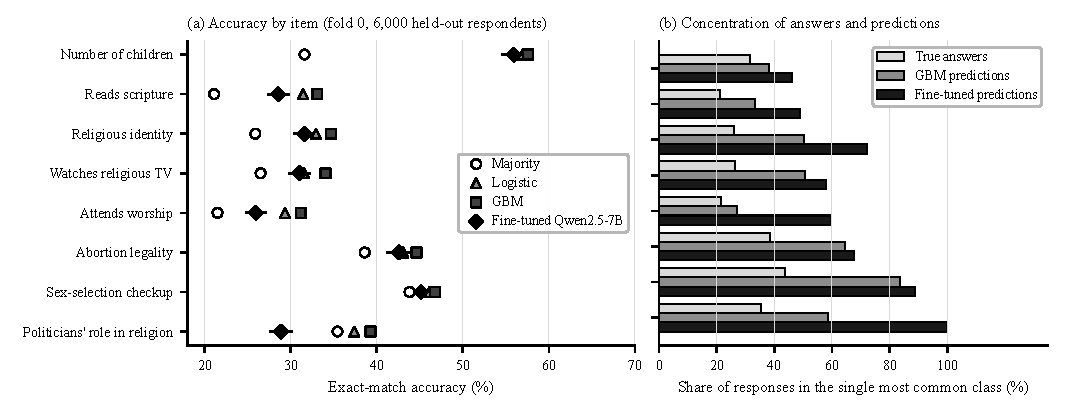
\includegraphics[width=\textwidth]{figs/fig_pew_items.pdf}
\caption{Pew fold-0 diagnostics. (a)~Accuracy per item and method; the bar on the fine-tuned marker is its 95\% respondent-bootstrap CI. (b)~Share of responses in the single most common class, for true answers and for the hard predictions of GBM and the fine-tuned model.}
\label{fig:pewitems}
\end{figure*}

\subsection{RQ3: what predictions do to distributions}

\begin{figure*}[!t]
\centering
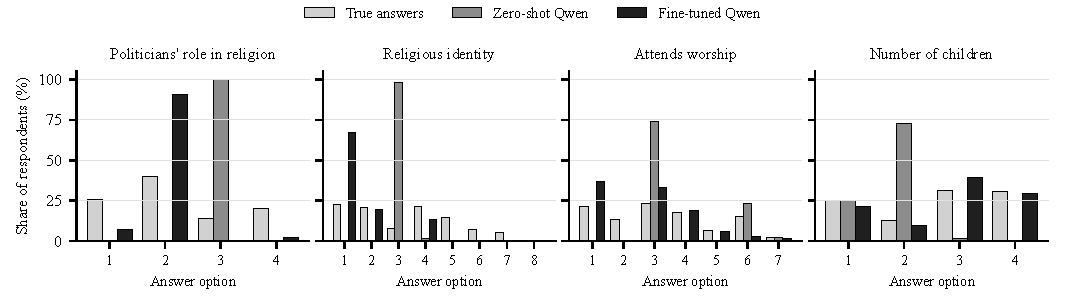
\includegraphics[width=\textwidth]{figs/fig_pew_dists.pdf}
\caption{Distribution of answers on four Pew items (200-respondent subset): true answers, zero-shot Qwen2.5-7B (chat), and the fine-tuned model. The zero-shot model selects one moderate option for nearly every respondent; the fine-tuned model recovers the dominant answer of the population but still concentrates.}
\label{fig:dists}
\end{figure*}

\begin{table}[!t]
\caption{Distributional diagnostics of hard predictions (Pew, means over items). Top share: fraction of responses in the most common class. TV: total variation distance between predicted and true answer distributions. SD ret.: dispersion retention. Gap infl.: median ratio of predicted to true between-group range.}
\label{tab:conc}
\centering
\footnotesize
\setlength{\tabcolsep}{2.6pt}
\begin{tabular}{@{}lrrrr@{}}
\toprule
\textbf{Predictor} & \textbf{Top share} & \textbf{TV} & \textbf{SD ret.} & \textbf{Gap infl.} \\
\midrule
True answers & 0.31 & 0.00 & 1.00 & 1.00 \\
Majority class & 1.00 & 0.69 & 0.00 & 0.0$\times$ \\
Logistic regression & 0.55 & 0.31 & 0.96 & 2.6$\times$ \\
Gradient boosting & 0.51 & 0.25 & 0.97 & 2.0$\times$ \\
Fine-tuned Qwen2.5-7B & 0.60 & 0.38 & 0.96 & 2.0$\times$ \\
\bottomrule
\end{tabular}
\end{table}

The fine-tuned model and both supervised classifiers concentrate answers (Table~\ref{tab:conc}): the mean share of responses in the most common class is 0.31 for true answers, 0.51 for GBM, and 0.68 for the fine-tuned model, which on ``politicians' role in religion'' emits one option for all 5{,}618 respondents (28.9\% vs.\ 35.4\% majority). Concentration does not, however, mean loss of spread: dispersion retention is 0.90 for the fine-tuned model and 0.97 for GBM. The more consequential distortion is between-group: hard predictions inflate the differences between demographic groups by 1.6$\times$ (fine-tuned), 2.0$\times$ (GBM), and 2.6$\times$ (logistic regression). Inflation therefore accompanies predicting the most likely answer for each profile, and the fine-tuned model shows the least of it.

The fine-tuned model is not a copy of a supervised classifier. It agrees with GBM on 63.5\% of answers ($\kappa=0.51$) and with logistic regression on 66.7\% ($\kappa=0.55$), whereas the two classifiers agree with each other on 76.5\% ($\kappa=0.70$). It departs from the majority-class prediction on 50.1\% of rows; on those rows it is correct 32.4\% of the time, against 20.9\% for the majority class and 38.1\% for GBM. Normalised subgroup-mean error falls from 0.343 (majority) to 0.208 (fine-tuned), a 39\% reduction, while GBM reaches 0.126. The zero-shot model behaves differently from all of these: it answers with a moderate option for nearly every respondent (Fig.~\ref{fig:dists}), with dispersion retention 0.54, and the total variation distance between its average predicted distribution and the true one is 0.55, against 0.06 for GBM's probabilities. It agrees with the fine-tuned model on only 8.5\% of rows.

\subsection{RQ4: subgroup fidelity}

\begin{figure}[!t]
\centering
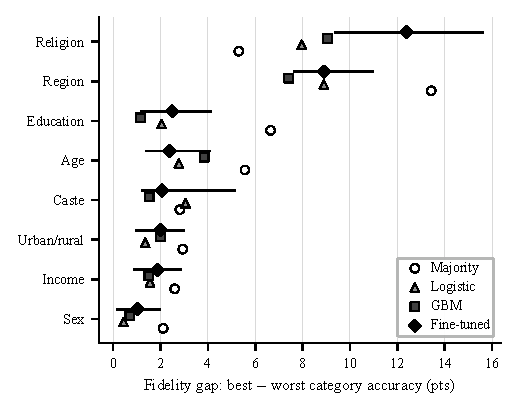
\includegraphics[width=\columnwidth]{figs/fig_pew_gaps.pdf}
\caption{Pew fidelity gaps (best minus worst category accuracy) by axis. The bar on the fine-tuned marker is its 95\% respondent-bootstrap CI. A majority-class predictor has gaps because groups differ in how common the modal answer is.}
\label{fig:gaps}
\end{figure}

\begin{table}[!t]
\caption{Pew fidelity gaps (accuracy points). FT is the fine-tuned model; $p$ is the permutation test of FT's gap; the last column is the paired difference in gap to GBM. Logistic regression is shown in Fig.~\ref{fig:gaps}.}
\label{tab:pewgaps}
\centering
\scriptsize
\setlength{\tabcolsep}{3.2pt}
\begin{tabular}{@{}lrrrrr@{}}
\toprule
\textbf{Axis} & \textbf{Maj.} & \textbf{GBM} & \textbf{FT gap [95\% CI]} & \textbf{$p$} & \textbf{FT$-$GBM [95\% CI]} \\
\midrule
Religion & 5.3 & 9.1 & 10.0 [7.3, 13.5] & $<$0.001 & +1.0 [$-$2.1, +4.0] \\
Region & 13.4 & 7.4 & 8.8 [7.1, 11.3] & $<$0.001 & +1.4 [+0.1, +3.5] \\
Education & 6.6 & 1.2 & 2.0 [0.9, 3.6] & 0.058 & +0.8 [$-$0.8, +2.2] \\
Age & 5.6 & 3.8 & 2.7 [1.7, 4.2] & 0.005 & $-$1.2 [$-$2.4, +0.5] \\
Caste & 2.8 & 1.5 & 3.4 [1.5, 6.3] & 0.071 & +1.9 [$-$1.5, +4.0] \\
Urban/rural & 2.9 & 2.0 & 1.3 [0.3, 2.2] & 0.012 & $-$0.7 [$-$1.5, +0.1] \\
Income & 2.6 & 1.5 & 1.7 [0.6, 2.7] & $<$0.001 & +0.2 [$-$0.6, +1.1] \\
Sex & 2.1 & 0.7 & 0.4 [0.0, 1.3] & 0.37 & $-$0.3 [$-$1.0, +0.5] \\
\bottomrule
\end{tabular}
\end{table}

\textbf{Pew (6{,}000 test respondents).} The fine-tuned model's gaps are reliably larger than chance for religion (12.4 points, 95\% CI 9.4--15.6), region (8.9), income, urban/rural, and education; these five remain significant after Holm correction across eight axes, whereas age ($p=0.022$), sex ($p=0.032$), and caste ($p=0.34$) do not (Fig.~\ref{fig:gaps}, Table~\ref{tab:pewgaps}). Within religion, accuracy is lowest for Buddhist respondents (27.2\%, 119 respondents) and highest for Muslim respondents (39.6\%); within region it is lowest in the West (30.9\%) and highest in Central India (39.8\%). Against GBM, no axis differs significantly (every interval for the paired difference contains or touches zero; largest: religion $+3.3$, CI 0.0 to $+6.5$). Against the majority class, conditioning narrows the gap for region ($-4.5$, CI $-6.6$ to $-2.0$), education ($-4.1$), and age ($-3.2$) but widens it for religion ($+7.1$, CI $+3.4$ to $+10.4$), so conditioning is not uniformly equalising.

\begin{table}[!t]
\caption{WVS-7 subgroup gaps in accuracy points, with permutation $p$ in parentheses and the detection threshold $\mathrm{Null}_{95}$ in brackets. Column headers give the number of respondents.}
\label{tab:wvsgaps}
\centering
\scriptsize
\setlength{\tabcolsep}{2.4pt}
\begin{tabular}{@{}lrrr@{}}
\toprule
\textbf{Axis} & \textbf{Gemini (30)} & \textbf{gpt-oss (40)} & \textbf{Qwen (120)} \\
\midrule
Region & 19.7 (.27) [26.0] & 7.9 (.93) [22.8] & 7.2 (.31) [10.9] \\
Age band & 8.8 (.82) [26.7] & 13.6 (.46) [23.1] & 4.0 (.71) [10.0] \\
Education & 13.2 (.08) [14.3] & 6.1 (.40) [10.8] & 2.1 (.74) [6.7] \\
Income & 10.2 (.33) [17.5] & 3.3 (.81) [12.2] & 6.4 (.08) [7.0] \\
Sex & 10.4 (.03) [9.4] & 0.1 (.98) [6.9] & 1.3 (.57) [4.5] \\
Urban/rural & 4.3 (.39) [9.5] & 2.4 (.53) [7.3] & 1.7 (.50) [4.5] \\
\bottomrule
\end{tabular}
\end{table}

\textbf{WVS-7.} With 30 to 40 respondents, observed gaps of 0.1 to 19.7 points sit below or near their detection thresholds (6.9 to 26.7 points; Table~\ref{tab:wvsgaps}); 11 of 12 permutation tests have $p>0.05$, and the exception (Gemini, sex, $p=0.026$) does not survive Holm correction. In the 120-respondent Qwen run, thresholds fall to 4.5 to 10.9 points, and again no axis is significant (smallest $p=$ 0.082, income). At this scale, gaps of the size most axes show on Pew (1 to 2.5 points) remain undetectable.

\section{Discussion}

\textbf{A concrete bar.} In both surveys an LLM conditioned on demographics does not exceed what a classifier on the same demographics provides, and without training data it does not exceed the majority class at the sample sizes tested. Any claim that LLM respondents add value for exact-match prediction should therefore be shown against a matched GBM and a majority-class baseline, both cheap to fit. The case for LLM respondents must rest on settings these baselines cannot reach, such as new questions or populations without respondent-level data.

\textbf{Fine-tuning transfers population structure.} The fine-tuned model scores 18.1 points above its own zero-shot control and 5.7 points above the majority class, cuts subgroup-mean error by 39\%, and closes 59\% of the majority-to-GBM distance, so parameter-efficient fine-tuning transfers real population structure that the zero-shot model does not carry. Its moderate agreement with GBM ($\kappa=0.51$) shows that the two make different errors, which suggests that combining them at the probability level could help; we do not test this.

\textbf{Inflation and concentration are not specific to LLMs.} Between-group inflation (1.6$\times$ to 2.6$\times$) and concentration appear for the fine-tuned model and for both supervised classifiers. Studies that report inflated segment gaps for LLMs should compare against a baseline that predicts the modal answer per profile, since such a baseline reproduces much of the effect. Population-level estimation should use sampled answers or answer-token probabilities rather than greedy decoding.

\textbf{Relation to distributional findings.} Miranda and Balbi~\cite{miranda2025} report that LLMs reproduce aggregate opinion distributions better than random forests when persona prompts carry attitudinal and moral variables (25 in total). We find the opposite for a zero-shot 7B model given nine demographics alone: its average predicted distribution is far from the truth (total variation 0.55 against 0.06 for GBM probabilities). Richer personas, larger models, or sampling rather than argmax may explain the difference; our data cannot separate these.

\textbf{Subgroup claims need a null.} At Pew scale gaps are measurable and mostly small (1 to 2.5 points) except for religion and region. At WVS scale a range statistic over a few respondents has a null median of 2.5 to 16 points. Because the majority baseline also has gaps, part of any accuracy gap reflects how predictable a group's answers are rather than model bias. We recommend reporting $\mathrm{Null}_{95}$ alongside gaps.

\section{Limitations}

\begin{itemize}
    \item \textbf{Different experiments.} The WVS zero-shot studies (15 items, 120 or fewer respondents) and the Pew fine-tuning study (8 items, 6{,}000 respondents) differ in survey, items, and model, so their accuracies are not comparable. Fine-tuning was carried out on Pew only, which has about 18 times as many respondents; a WVS fine-tuning comparison is left to future work.
    \item \textbf{Subset-based control.} The zero-shot controls and the local WVS run use nested random respondent subsets (compute-limited), and the intervals reflect their sizes. The adapter was not re-scored locally, since 4-bit MLX quantization differs from the bitsandbytes NF4 used in training, so the fine-tuned model's results are hard predictions from the original run and no fine-tuned probabilities (NLL, calibration) are reported.
    \item \textbf{Single run.} Fine-tuning used one fold, one seed, one epoch, and a full-sequence loss; an answer-only objective, other seeds, or more epochs may change results.
    \item \textbf{Item coverage.} The eight Pew items concern religion and fertility; the 15 WVS items are a fixed subset of 144. Results may not transfer to other topics.
    \item \textbf{Models and data.} The API models are free-tier, non-frontier systems; contamination is possible since both surveys are public; the WVS interview-language field is constant, so no language axis could be tested.
    \item \textbf{Interpretation.} Accuracy gaps conflate predictability with bias and are not causal claims about a model.
\end{itemize}

\textbf{Ethical considerations.} Both datasets are public and de-identified, and we do not redistribute WVS microdata. Simulated respondents should not replace sampling of real people, particularly for subgroups where accuracy was lower.

\section{Conclusion and Future Work}

On two Indian surveys, a baseline-matched protocol shows that zero-shot LLM respondents match but do not exceed the majority class, that QLoRA fine-tuning on respondent-level data lifts a 7B model from chance level (17.5\%) to 36.1\%, 59\% of the way from the majority class to gradient boosting, and that hard predictions of the fine-tuned model and of both supervised classifiers inflate between-group differences, so such effects must be read against a baseline. Subgroup gaps in religion and region are real and comparable to a supervised classifier's, and WVS-scale samples cannot test subgroup claims. We provide detection thresholds, the evaluation pipeline, and scripts that scale each experiment (\texttt{SCALE\_UP.md}).

Future work includes scoring the adapter with its own probabilities (distribution-level fidelity and ensembling with GBM) on a CUDA GPU with the provided script, all five folds with multiple seeds, an answer-only training objective, and a WVS fine-tuning comparison with larger models.

\section*{Data and Code Availability}
Code and prompts are in the project repository (\url{https://github.com/bhanujjj/silicon-sampling-capstone}; branches \texttt{lab-package} and \texttt{pew-dataset-training}); the analysis scripts, including the local MLX and CUDA runners used here, are distributed with this paper's source. WVS-7 must be obtained from the WVS Association under its terms; the Pew data are available from Pew Research Center.

\section*{Acknowledgment}
The authors thank their university's AI Lab for GPU access.

\begin{thebibliography}{99}

\bibitem{argyle2023}
L.~P. Argyle, E.~C. Busby, N.~Fulda, J.~R. Gubler, C.~Rytting, and D.~Wingate, ``Out of one, many: Using language models to simulate human samples,'' \emph{Political Analysis}, vol.~31, no.~3, pp. 337--351, 2023.

\bibitem{santurkar2023}
S.~Santurkar, E.~Durmus, F.~Ladhak, C.~Lee, P.~Liang, and T.~Hashimoto, ``Whose opinions do language models reflect?'' in \emph{Proc. 40th Int. Conf. Machine Learning (ICML)}, 2023.

\bibitem{durmus2023}
E.~Durmus \emph{et al.}, ``Towards measuring the representation of subjective global opinions in language models,'' arXiv:2306.16388, 2023.

\bibitem{bisbee2024}
J.~Bisbee, J.~D. Clinton, C.~Dorff, B.~Kenkel, and J.~M. Larson, ``Synthetic replacements for human survey data? The perils of large language models,'' \emph{Political Analysis}, vol.~32, 2024.

\bibitem{aher2023}
G.~Aher, R.~I. Arriaga, and A.~T. Kalai, ``Using large language models to simulate multiple humans and replicate human subject studies,'' in \emph{Proc. 40th Int. Conf. Machine Learning (ICML)}, 2023.

\bibitem{dillion2023}
D.~Dillion, N.~Tandon, Y.~Gu, and K.~Gray, ``Can AI language models replace human participants?'' \emph{Trends in Cognitive Sciences}, vol.~27, no.~7, pp. 597--600, 2023.

\bibitem{shankar2026}
H.~Shankar, V.~S.~P., S.~Margapuri, D.~Mazumder, P.~Kumaraguru, and A.~Chakraborty, ``Mind the gap: Pitfalls of LLM alignment with Asian public opinion,'' arXiv:2603.06264, 2026.

\bibitem{kim2023}
J.~Kim and B.~Lee, ``AI-augmented surveys: Leveraging large language models and surveys for opinion prediction,'' arXiv:2305.09620, 2023.

\bibitem{suh2025}
J.~Suh, E.~Jahanparast, S.~Moon, M.~Kang, and S.~Chang, ``Language model fine-tuning on scaled survey data for predicting distributions of public opinions,'' arXiv:2502.16761, 2025.

\bibitem{cao2025}
Y.~Cao, H.~Liu, A.~Arora, I.~Augenstein, P.~R\"{o}ttger, and D.~Hershcovich, ``Specializing large language models to simulate survey response distributions for global populations,'' in \emph{Proc. NAACL}, 2025.

\bibitem{zhao2024}
W.~Zhao, D.~Mondal, N.~Tandon, D.~Dillion, K.~Gray, and Y.~Gu, ``WorldValuesBench: A large-scale benchmark dataset for multi-cultural value awareness of language models,'' in \emph{Proc. LREC-COLING}, 2024.

\bibitem{sun2024}
S.~Sun \emph{et al.}, ``Random silicon sampling: Simulating human sub-population opinion using a large language model based on group-level demographic information,'' arXiv:2402.18144, 2024.

\bibitem{krsteski2025}
S.~Krsteski, G.~Russo, S.~Chang, R.~West, and K.~Gligori\'{c}, ``Valid survey simulations with limited human data: The roles of prompting, fine-tuning, and rectification,'' arXiv:2510.11408, 2025.

\bibitem{miranda2025}
F.~Miranda and P.~P. Balbi, ``Simulating public opinion: Comparing distributional and individual-level predictions from LLMs and random forests,'' \emph{Entropy}, Sep. 2025.

\bibitem{chen2026}
Z.~Chen, D.~Zhu, and L.~N. Zheng, ``When synthetic users fail: A cross-domain benchmark of LLM-simulated human survey responses,'' arXiv:2607.26348, 2026.

\bibitem{ziaei2026}
R.~Ziaei, ``The limits of simulated societies: How post-training and survey fine-tuning erase cross-cultural variance,'' arXiv:2609.25760, 2026.

\bibitem{wvs7}
C.~Haerpfer \emph{et al.} (eds.), \emph{World Values Survey: Round Seven, Country-Pooled Datafile Version 6.0}. Madrid, Spain and Vienna, Austria: JD Systems Institute \& WVSA Secretariat, 2022, doi:10.14281/18241.24.

\bibitem{pew2021}
Pew Research Center, ``Religion in India: Tolerance and segregation,'' Jun. 2021.

\bibitem{pedregosa2011}
F.~Pedregosa \emph{et al.}, ``Scikit-learn: Machine learning in Python,'' \emph{J. Mach. Learn. Res.}, vol.~12, pp. 2825--2830, 2011.

\bibitem{gptoss2025}
OpenAI, ``gpt-oss-120b and gpt-oss-20b model card,'' 2025.

\bibitem{qwen2025}
Qwen Team, ``Qwen2.5 technical report,'' arXiv:2412.15115, 2024.

\bibitem{mlx2023}
Apple Machine Learning Research, ``MLX: An array framework for Apple silicon,'' 2023.

\bibitem{dettmers2023}
T.~Dettmers, A.~Pagnoni, A.~Holtzman, and L.~Zettlemoyer, ``QLoRA: Efficient finetuning of quantized LLMs,'' in \emph{Advances in Neural Information Processing Systems (NeurIPS)}, vol.~36, 2023.

\bibitem{hu2022}
E.~J. Hu \emph{et al.}, ``LoRA: Low-rank adaptation of large language models,'' in \emph{Proc. Int. Conf. Learning Representations (ICLR)}, 2022.

\bibitem{phipson2010}
B.~Phipson and G.~K. Smyth, ``Permutation $p$-values should never be zero: Calculating exact $p$-values when permutations are randomly drawn,'' \emph{Stat. Appl. Genet. Mol. Biol.}, vol.~9, no.~1, art.~39, 2010.

\bibitem{efron1993}
B.~Efron and R.~J. Tibshirani, \emph{An Introduction to the Bootstrap}. New York, NY, USA: Chapman \& Hall, 1993.

\bibitem{holm1979}
S.~Holm, ``A simple sequentially rejective multiple test procedure,'' \emph{Scand. J. Statist.}, vol.~6, no.~2, pp. 65--70, 1979.

\bibitem{cohen1960}
J.~Cohen, ``A coefficient of agreement for nominal scales,'' \emph{Educ. Psychol. Meas.}, vol.~20, no.~1, pp. 37--46, 1960.

\end{thebibliography}

\end{document}
